

\tikzset{every picture/.style={line width=0.75pt}} %set default line width to 0.75pt        

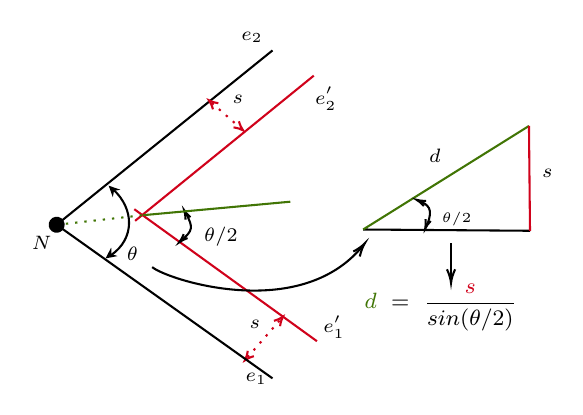
\begin{tikzpicture}[x=0.75pt,y=0.75pt,yscale=-1,xscale=1]
%uncomment if require: \path (0,300); %set diagram left start at 0, and has height of 300

%Straight Lines [id:da040119542158275845] 
\draw    (74.96,146.08) -- (178.96,62.08) ;
%Curve Lines [id:da8293026312934688] 
\draw    (101.21,160.68) .. controls (112.52,152.9) and (112.54,138.62) .. (102.31,129.15) ;
\draw [shift={(100.03,127.25)}, rotate = 44.62] [fill={rgb, 255:red, 0; green, 0; blue, 0 }  ][line width=0.08]  [draw opacity=0] (5.36,-2.57) -- (0,0) -- (5.36,2.57) -- (3.56,0) -- cycle    ;
\draw [shift={(98.5,162.3)}, rotate = 323.23] [fill={rgb, 255:red, 0; green, 0; blue, 0 }  ][line width=0.08]  [draw opacity=0] (5.36,-2.57) -- (0,0) -- (5.36,2.57) -- (3.56,0) -- cycle    ;
%Straight Lines [id:da044371428727159934] 
\draw [color={rgb, 255:red, 208; green, 2; blue, 27 }  ,draw opacity=1 ] [dash pattern={on 0.84pt off 2.51pt}]  (149.79,87.4) -- (163.27,99.25) ;
\draw [shift={(164.77,100.58)}, rotate = 221.34] [color={rgb, 255:red, 208; green, 2; blue, 27 }  ,draw opacity=1 ][line width=0.75]    (4.37,-1.96) .. controls (2.78,-0.92) and (1.32,-0.27) .. (0,0) .. controls (1.32,0.27) and (2.78,0.92) .. (4.37,1.96)   ;
\draw [shift={(148.29,86.08)}, rotate = 41.34] [color={rgb, 255:red, 208; green, 2; blue, 27 }  ,draw opacity=1 ][line width=0.75]    (4.37,-1.96) .. controls (2.78,-0.92) and (1.32,-0.27) .. (0,0) .. controls (1.32,0.27) and (2.78,0.92) .. (4.37,1.96)   ;
%Straight Lines [id:da7636321254468201] 
\draw [color={rgb, 255:red, 208; green, 2; blue, 27 }  ,draw opacity=1 ] [dash pattern={on 0.84pt off 2.51pt}]  (166.94,209.91) -- (182.69,191.85) ;
\draw [shift={(184,190.35)}, rotate = 131.09] [color={rgb, 255:red, 208; green, 2; blue, 27 }  ,draw opacity=1 ][line width=0.75]    (4.37,-1.96) .. controls (2.78,-0.92) and (1.32,-0.27) .. (0,0) .. controls (1.32,0.27) and (2.78,0.92) .. (4.37,1.96)   ;
\draw [shift={(165.63,211.41)}, rotate = 311.09] [color={rgb, 255:red, 208; green, 2; blue, 27 }  ,draw opacity=1 ][line width=0.75]    (4.37,-1.96) .. controls (2.78,-0.92) and (1.32,-0.27) .. (0,0) .. controls (1.32,0.27) and (2.78,0.92) .. (4.37,1.96)   ;
%Straight Lines [id:da4959645731484468] 
\draw [color={rgb, 255:red, 208; green, 2; blue, 27 }  ,draw opacity=1 ]   (112.37,138.58) -- (200.37,202.18) ;
%Straight Lines [id:da37518220757042164] 
\draw [color={rgb, 255:red, 208; green, 2; blue, 27 }  ,draw opacity=1 ]   (112.77,144.18) -- (198.86,74.23) ;
%Straight Lines [id:da03224684631327923] 
\draw [color={rgb, 255:red, 65; green, 117; blue, 5 }  ,draw opacity=1 ] [dash pattern={on 0.84pt off 2.51pt}]  (74.96,146.08) -- (116.52,141.47) ;
%Curve Lines [id:da6196010222690171] 
\draw    (135.54,153.21) .. controls (140.32,148.98) and (140.94,147.45) .. (137.35,140.79) ;
\draw [shift={(136.39,139.06)}, rotate = 64.81] [color={rgb, 255:red, 0; green, 0; blue, 0 }  ][line width=0.75]    (4.37,-1.32) .. controls (2.78,-0.56) and (1.32,-0.12) .. (0,0) .. controls (1.32,0.12) and (2.78,0.56) .. (4.37,1.32)   ;
\draw [shift={(133.97,154.58)}, rotate = 315.94] [color={rgb, 255:red, 0; green, 0; blue, 0 }  ][line width=0.75]    (4.37,-1.32) .. controls (2.78,-0.56) and (1.32,-0.12) .. (0,0) .. controls (1.32,0.12) and (2.78,0.56) .. (4.37,1.32)   ;
%Straight Lines [id:da6848739970418427] 
\draw    (74.96,146.08) -- (178.96,220.08) ;
\draw [shift={(74.96,146.08)}, rotate = 35.43] [color={rgb, 255:red, 0; green, 0; blue, 0 }  ][fill={rgb, 255:red, 0; green, 0; blue, 0 }  ][line width=0.75]      (0, 0) circle [x radius= 3.35, y radius= 3.35]   ;
%Straight Lines [id:da19412102153259814] 
\draw [color={rgb, 255:red, 65; green, 117; blue, 5 }  ,draw opacity=1 ]   (116.52,141.47) -- (187.52,134.97) ;
%Straight Lines [id:da08103351548467064] 
\draw    (222.62,148.36) -- (303.02,148.97) ;
%Straight Lines [id:da7746295407362944] 
\draw [color={rgb, 255:red, 65; green, 117; blue, 5 }  ,draw opacity=1 ]   (222.62,148.36) -- (302.52,98.47) ;
%Straight Lines [id:da6727152009251198] 
\draw [color={rgb, 255:red, 208; green, 2; blue, 27 }  ,draw opacity=1 ]   (302.52,98.47) -- (303.02,148.97) ;
%Curve Lines [id:da10208771376844283] 
\draw    (253.39,146.1) .. controls (256.77,138.23) and (253.6,136.34) .. (250.18,134.84) ;
\draw [shift={(248.39,134.06)}, rotate = 23.36] [color={rgb, 255:red, 0; green, 0; blue, 0 }  ][line width=0.75]    (4.37,-1.32) .. controls (2.78,-0.56) and (1.32,-0.12) .. (0,0) .. controls (1.32,0.12) and (2.78,0.56) .. (4.37,1.32)   ;
\draw [shift={(252.52,147.97)}, rotate = 288.75] [color={rgb, 255:red, 0; green, 0; blue, 0 }  ][line width=0.75]    (4.37,-1.32) .. controls (2.78,-0.56) and (1.32,-0.12) .. (0,0) .. controls (1.32,0.12) and (2.78,0.56) .. (4.37,1.32)   ;
%Curve Lines [id:da6567322872014665] 
\draw    (120.98,166.47) .. controls (127.97,172.41) and (192.16,193.54) .. (222.55,156.12) ;
\draw [shift={(223.46,154.97)}, rotate = 127.57] [color={rgb, 255:red, 0; green, 0; blue, 0 }  ][line width=0.75]    (6.56,-1.97) .. controls (4.17,-0.84) and (1.99,-0.18) .. (0,0) .. controls (1.99,0.18) and (4.17,0.84) .. (6.56,1.97)   ;
%Straight Lines [id:da8309736780448946] 
\draw    (264.97,155.1) -- (264.97,172.1) ;
\draw [shift={(264.97,174.1)}, rotate = 270] [color={rgb, 255:red, 0; green, 0; blue, 0 }  ][line width=0.75]    (6.56,-1.97) .. controls (4.17,-0.84) and (1.99,-0.18) .. (0,0) .. controls (1.99,0.18) and (4.17,0.84) .. (6.56,1.97)   ;

% Text Node
\draw (147.6,173.07) node [anchor=north west][inner sep=0.75pt]   [align=left] {$ $};
% Text Node
\draw (107.29,155.25) node [anchor=north west][inner sep=0.75pt]  [font=\scriptsize] [align=left] {$\displaystyle \theta $};
% Text Node
\draw (158.28,82.12) node [anchor=north west][inner sep=0.75pt]  [font=\scriptsize] [align=left] {$\displaystyle s$};
% Text Node
\draw (166.38,190.72) node [anchor=north west][inner sep=0.75pt]  [font=\scriptsize] [align=left] {$\displaystyle s$};
% Text Node
\draw (144.57,145.48) node [anchor=north west][inner sep=0.75pt]  [font=\scriptsize] [align=left] {$\displaystyle \theta /2$};
% Text Node
\draw (61.5,150.26) node [anchor=north west][inner sep=0.75pt]  [font=\scriptsize] [align=left] {$\displaystyle N$};
% Text Node
\draw (164.5,216.26) node [anchor=north west][inner sep=0.75pt]  [font=\scriptsize] [align=left] {$\displaystyle e_{1}$};
% Text Node
\draw (162.5,51.62) node [anchor=north west][inner sep=0.75pt]  [font=\scriptsize] [align=left] {$\displaystyle e_{2}$};
% Text Node
\draw (202,188.26) node [anchor=north west][inner sep=0.75pt]  [font=\scriptsize] [align=left] {$\displaystyle e'_{1}$};
% Text Node
\draw (198,78.26) node [anchor=north west][inner sep=0.75pt]  [font=\scriptsize] [align=left] {$\displaystyle e'_{2}$};
% Text Node
\draw (259.07,138.48) node [anchor=north west][inner sep=0.75pt]  [font=\tiny] [align=left] {$\displaystyle \theta /2$};
% Text Node
\draw (307.38,117.86) node [anchor=north west][inner sep=0.75pt]  [font=\scriptsize] [align=left] {$\displaystyle s$};
% Text Node
\draw (252.88,107.86) node [anchor=north west][inner sep=0.75pt]  [font=\scriptsize] [align=left] {$\displaystyle d$};
% Text Node
\draw (221.8,173) node [anchor=north west][inner sep=0.75pt]  [font=\footnotesize] [align=left] {$\displaystyle \textcolor[rgb]{0.25,0.46,0.02}{d} \ =\ \frac{\textcolor[rgb]{0.82,0.01,0.11}{s}}{sin( \theta /2)}$};


\end{tikzpicture}
